\documentclass[tikz,border=12pt]{standalone}
\usepackage[T1]{fontenc}
\usepackage{tgheros}
\usepackage{sfmath}
\usepackage{amsmath}
\usepackage{tikz}
\usetikzlibrary{arrows.meta,positioning,shapes.geometric,fit,backgrounds,calc}
\usepackage{xcolor}

\renewcommand{\familydefault}{\sfdefault}

\definecolor{crimson}{HTML}{A51C30}
\definecolor{crimsonlight}{HTML}{FEF2F2}
\definecolor{darkblue}{HTML}{1F407A}
\definecolor{bluelight}{HTML}{F0F4FA}
\definecolor{petrol}{HTML}{007A87}
\definecolor{petrollight}{HTML}{EDF7F7}
\definecolor{slate}{HTML}{475569}
\definecolor{mutedslate}{HTML}{64748B}
\definecolor{bordercolor}{HTML}{CBD5E1}

\begin{document}
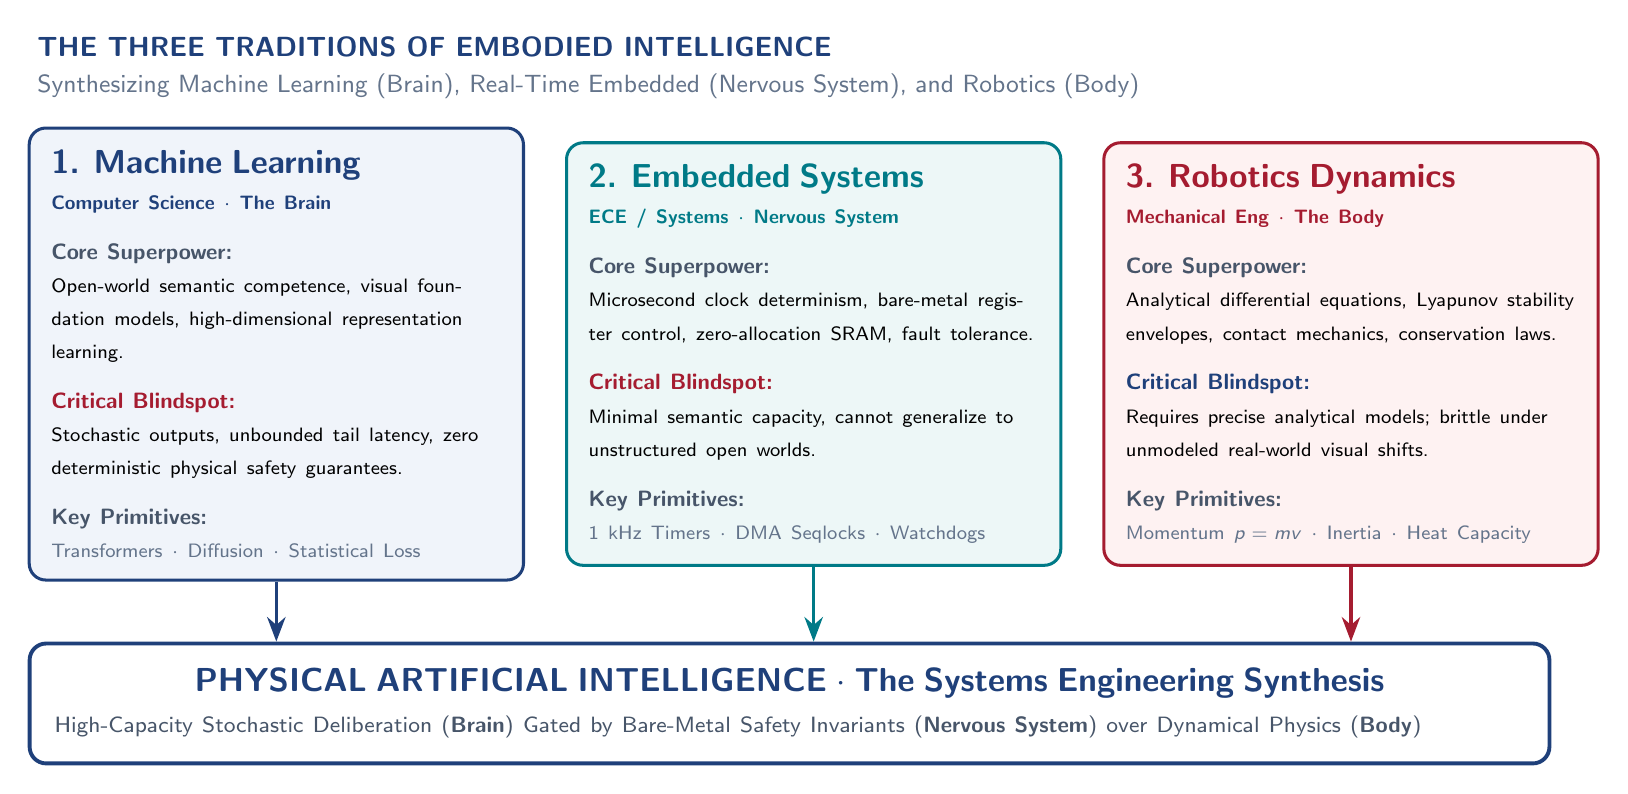
\begin{tikzpicture}[
  font=\sffamily,
  >=Stealth,
  node distance=0.20in,
  columncard/.style 2 args={
    draw=#1,
    fill=#2,
    rounded corners=6pt,
    line width=1.1pt,
    inner sep=8pt,
    text width=2.25in,
    align=left
  }
]

  % Title Block
  \node[anchor=west, font=\sffamily\bfseries\normalsize, text=darkblue] at (0, 0.35in) {THE THREE TRADITIONS OF EMBODIED INTELLIGENCE};
  \node[anchor=west, font=\sffamily\small, text=mutedslate] at (0, 0.15in) {Synthesizing Machine Learning (Brain), Real-Time Embedded (Nervous System), and Robotics (Body)};

  % Column 1: Computer Science / ML (The Brain)
  \node[columncard={darkblue}{bluelight}, anchor=north west] (c1) at (0, -0.05in) {
    \textbf{\color{darkblue}\large 1. Machine Learning}\\[1pt]
    {\scriptsize\bfseries\color{darkblue} Computer Science $\cdot$ The Brain}\\[6pt]
    \textbf{\color{slate}\footnotesize Core Superpower:}\\
    {\scriptsize Open-world semantic competence, visual foundation models, high-dimensional representation learning.}\\[6pt]
    \textbf{\color{crimson}\footnotesize Critical Blindspot:}\\
    {\scriptsize Stochastic outputs, unbounded tail latency, zero deterministic physical safety guarantees.}\\[6pt]
    \textbf{\color{slate}\footnotesize Key Primitives:}\\
    {\scriptsize\color{mutedslate} Transformers $\cdot$ Diffusion $\cdot$ Statistical Loss}
  };

  % Column 2: Embedded Systems / ECE (The Nervous System)
  \node[columncard={petrol}{petrollight}, right=0.20in of c1] (c2) {
    \textbf{\color{petrol}\large 2. Embedded Systems}\\[1pt]
    {\scriptsize\bfseries\color{petrol} ECE / Systems $\cdot$ Nervous System}\\[6pt]
    \textbf{\color{slate}\footnotesize Core Superpower:}\\
    {\scriptsize Microsecond clock determinism, bare-metal register control, zero-allocation SRAM, fault tolerance.}\\[6pt]
    \textbf{\color{crimson}\footnotesize Critical Blindspot:}\\
    {\scriptsize Minimal semantic capacity, cannot generalize to unstructured open worlds.}\\[6pt]
    \textbf{\color{slate}\footnotesize Key Primitives:}\\
    {\scriptsize\color{mutedslate} 1 kHz Timers $\cdot$ DMA Seqlocks $\cdot$ Watchdogs}
  };

  % Column 3: Mechanical Engineering / Robotics Dynamics (The Body)
  \node[columncard={crimson}{crimsonlight}, right=0.20in of c2] (c3) {
    \textbf{\color{crimson}\large 3. Robotics Dynamics}\\[1pt]
    {\scriptsize\bfseries\color{crimson} Mechanical Eng $\cdot$ The Body}\\[6pt]
    \textbf{\color{slate}\footnotesize Core Superpower:}\\
    {\scriptsize Analytical differential equations, Lyapunov stability envelopes, contact mechanics, conservation laws.}\\[6pt]
    \textbf{\color{darkblue}\footnotesize Critical Blindspot:}\\
    {\scriptsize Requires precise analytical models; brittle under unmodeled real-world visual shifts.}\\[6pt]
    \textbf{\color{slate}\footnotesize Key Primitives:}\\
    {\scriptsize\color{mutedslate} Momentum $p=mv$ $\cdot$ Inertia $\cdot$ Heat Capacity}
  };

  % Base Platform: Physical AI Synthesis
  \node[draw=darkblue, fill=white, rounded corners=6pt, line width=1.4pt, inner sep=9pt, text width=7.35in, below=0.30in of c1.south west, anchor=north west] (base) {
    \centering
    \textbf{\color{darkblue}\large PHYSICAL ARTIFICIAL INTELLIGENCE $\cdot$ The Systems Engineering Synthesis}\\[3pt]
    {\footnotesize\color{slate}High-Capacity Stochastic Deliberation (\textbf{Brain}) Gated by Bare-Metal Safety Invariants (\textbf{Nervous System}) over Dynamical Physics (\textbf{Body})}
  };

  % Connecting Arrows from Columns down into the Base
  \draw[->, line width=1.3pt, darkblue] (c1.south) -- (c1.south |- base.north);
  \draw[->, line width=1.3pt, petrol] (c2.south) -- (c2.south |- base.north);
  \draw[->, line width=1.3pt, crimson] (c3.south) -- (c3.south |- base.north);

\end{tikzpicture}
\end{document}
